
%%%%%%%%%%%%%%%%%%%%%%%%%%%%%%%%%%%%%%%%%%%%%%%%%%%%%%%%%%%%%%%%%%%%
%% I, the copyright holder of this work, release this work into the
%% public domain. This applies worldwide. In some countries this may
%% not be legally possible; if so: I grant anyone the right to use
%% this work for any purpose, without any conditions, unless such
%% conditions are required by law.
%%%%%%%%%%%%%%%%%%%%%%%%%%%%%%%%%%%%%%%%%%%%%%%%%%%%%%%%%%%%%%%%%%%%

\documentclass[compress]{beamer}
\usetheme[faculty=phil, navigation, microtype]{fibeamer}
%\usetheme[logo=resources/NOKIA]{fibeamer}
\useoutertheme{miniframes}
\setbeamercolor{section in head/foot}{fg=white, bg=fibeamer@blue}
\usepackage[francais]{babel}
\usepackage[utf8]{inputenc}
\usepackage[T1]{fontenc}
%\title{Requêtes probabilistes et pondérées en logique d'arbre de calcul %
\includegraphics[width=0.25\linewidth]{fibeamer/logo/mu/storm}
\title{Synthèse multi-objectifs dans les processus décisionnels de Markov} %% that will be typeset on the
%\subtitle{Presentation Subtitle} %% title page.
\author{Florent Delgrange}
\vspace{0.5cm}
\subtitle{\normalsize UMONS \\ Faculté des Sciences \\ Mab2 Science Informatique}
\date{\today}
%% These additional packages are used within the document:
\usepackage{ragged2e}  % `\justifying` text
\usepackage{bbold}
\usepackage{booktabs}  % Tables
\usepackage{centernot}
\usepackage{tabularx}
\usepackage{tikz}      % Diagrams
\usetikzlibrary{calc, shapes, backgrounds}
\usepackage{arevtext,arevmath}
\usepackage{verbatim}
\usepackage{amsmath, amssymb}
\usepackage{url}       % `\url`s
\usepackage{listings}
\usepackage{changepage}
\usepackage{cprotect}
\usepackage{caption}
\usepackage{graphicx}
\usepackage{minted}
\usepackage{biblatex}
\usepackage{mathtools}
\usepackage{multicol}
\frenchspacing

%% PRISM CODE LISTING *********************************************

\definecolor{prismgreen}{rgb}{0, 0.6, 0}

\lstdefinelanguage{Prism}{ % syntax highlight via font
	basicstyle=\color{red}\tiny\ttfamily, % small true type font (like courier)
	keywords=
	{bool,C,ceil,const,ctmc,double,dtmc,endinit,endmodule,endrewards, endsystem,F,false,floor,formula,G,global,I,init,int,label,max,mdp,min,
	module,nondeterministic,P,Pmin,Pmax,prob,probabilistic,R,rate,rewards, Rmin,Rmax,S,stochastic,system,true,U,X},
	keywordstyle={\bfseries\color{black}},
	numberstyle=\tiny\color{black},
	comment=[l] {//}, morecomment=[s]{/*}{*/}, % single and multi-line
	commentstyle= \color{prismgreen}, % dark green
	tabsize=4, % tab treatment (going to be fixed in Prism)
	captionpos=b, % put captions at the bottom
	escapechar=@ % write LaTeX comments escaped by @ symbol
}

%define command \prism with one argument for inline printing of \prism code
\newcommand{\prism}[1]{\lstinline[language=Prism,basicstyle=\small
	\ttfamily]|#1|}

%% END PRISM CODE LISTING


\definecolor{DarkOrange}{HTML}{FF8C00}

\bibliography{bib}
\begin{document}
  \begin{frame}[plain]
    \maketitle
  \end{frame}

  \AtBeginSection[]
    {
      %  \begin{frame}<beamer>
      %  \frametitle{Plan}
      %  \tableofcontents[currentsection]
      %  \end{frame}
      \begin{frame}{\contentsname}
      \vspace{-0.05\linewidth}
      %\footnotesize
      \begin{multicols}{2}
      \tableofcontents[currentsection]
      \end{multicols}
      \end{frame}
    }

\section{SP-G}
\subsection{Motivations}
\begin{frame}{Borne supérieure stricte dans un MDP}
  Soit $\mathcal{M} = (S, A, \Delta, w)$, un MDP, $s \in S$, un état de $\mathcal{M}$ et $T \subseteq S$, un sous-ensemble d'états cibles.\\ On va définir une stratégie $\sigma$ qui
    \textbf{\color{fibeamer@orange}garantit d'atteindre $T$ depuis $s$ avec un coût inférieur à un seuil $l$:}
    \begin{itemize}
      \item[$\leadsto$] $\forall \pi \in Paths^\sigma(s), \; TS^T(\pi) \leq l$
      \item[$\equiv$] $\mathbb{P}_s^\sigma (\Diamond_{\leq l} T ) = 1$
    \end{itemize}
%   \item minimise l'espérance du coût de l'accessibilité à $T$ tout en ayant une garantie de ne pas dépasser un seuil de coût $l$.
%     \begin{align*}
%       & \min_\sigma \quad \mathbb{E}_s^\sigma(\Diamond T) & \text{tel que} && \mathbb{P}_s^\sigma(\Diamond_{\leq l} T) = 1&
%     \end{align*}
On veut donc assurer une \textbf{\color{fibeamer@orange}borne supérieure stricte}
lors de l'accessibilité à $T$.
\end{frame}

\begin{frame}{Borne supérieure stricte dans un MDP}{Remarque}
  \begin{itemize}
    \item $\forall \pi \in Paths^\sigma(s), \; TS^T(\pi) \leq l$
    \item $\mathbb{P}_s^\sigma (\Diamond_{\leq l} T ) = 1$ \\
  \end{itemize}
  {\small {\color{fibeamer@orange}$w:A \rightarrow \mathbb{N}_0$} $\implies$ Ces deux propositions sont équivalentes ! \\
  En effet, le problème \textit{SSP-P} induit un \textbf{\color{fibeamer@orange}dépliage} de $\mathcal{M}$, dont le graphe sous-jacent est un DAG (si on ne considère pas les les états terminaux).}
  \begin{center}
    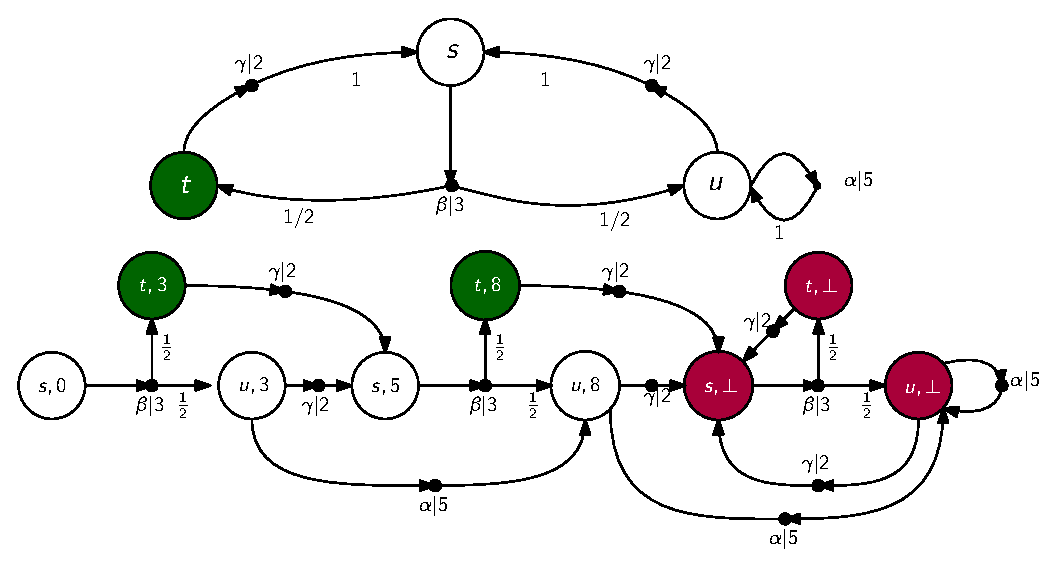
\includegraphics[width=0.7\linewidth]{resources/unfolding}
  \end{center}
\end{frame}

\begin{frame}{Problème du plus court chemin dans un jeu}
    Assurer une borne supérieure stricte lors de l'accessibilité à $T$  \\ {\color{fibeamer@blue}$\leadsto$} Problème \textbf{\color{fibeamer@orange}SP-G} (\textit{Shortest path game problem}) \\
    \`A chaque étape,
    \begin{itemize}
      \item \textbf{Joueur 1} : choisit l'action par stratégie
      \item \textbf{Joueur 2} : choisit le successeur $s'$, i.e., l'état qui mène au pire cas en terme de somme tronquée
    \end{itemize}
\end{frame}

\subsection{Définition}
\begin{frame}{Problème du plus court chemin dans un jeu}
  \begin{definition}[SP-G]
    Soient $\mathcal{M} = (S, A, \Delta, w)$ un MDP, $s \in S$, un état de $\mathcal{M}$, $T \subseteq S$, un sous-ensemble d'états cibles et un seuil $l \in \mathbb{N}$. \\
    Le problème \textit{\color{fibeamer@orange}SP-G} consiste à décider s'il existe une stratégie $\sigma$ pour laquelle
    \[
      \forall \pi \in Paths^\sigma(s), \; TS^T(\pi) \leq l
    \]
    \[
      \equiv \quad \mathbb{P}_s^\sigma(\Diamond_{\leq l} T) = 1
    \]
  \end{definition}
  \begin{itemize}
    \item peut être décidé en temps polynomial
    \item stratégie sans mémoire
  \end{itemize}
\end{frame}

\subsection{Algorithme}
\begin{frame}{Problème du plus court chemin dans un jeu}{Hypothèses}
\[ w : A \rightarrow \mathbb{N}_0 \]
  \begin{itemize}
    \item Les coûts sont strictement positifs
    \item[$\leadsto$] Pas de cycle pendant la minimisation de $TS^T$
    \begin{itemize}
      \item pas d'intérêt car poids strictement positifs
    \end{itemize}
    \item[$\leadsto$] \alert{$TS^T = \infty$ si les cycles ne peuvent pas être évités}
  \end{itemize}
\end{frame}

\begin{frame}{SP-G : Programmation dynamique}{Algorithme}
    %Soient $\mathcal{M} = (S, A, \Delta, w)$ un MDP, $s \in S$, un état de $\mathcal{M}$, $T \subseteq S$, un sous-ensemble d'états cibles et un seuil $l \in \mathbb{N}$.\\
    $\mathbb{C}(s, i)$ est le plus court chemin jusque $T$ depuis $s$, après $i$ étapes, $\forall 0 \leq i \leq n, \; n = |S|$ (pas de cycle).% \[ \]
    \\ $ $ \vspace{-0.03\linewidth}\\
      \textbf{\color{fibeamer@orange}Initialisation : }
      \begin{itemize}
        \item $\forall t \in T$, $\mathbb{C}(t, 0) = 0$
        \item $\forall s \in S$, $\mathbb{C}(s, T) = \infty$
      \end{itemize}
      Soit $k \in \mathbb{N}$ tel que $0 < k < n$. Supposons que $\mathbb{C}(s, k-1)$ a déjà été calculé pour tout $s \in S$.
        Alors, pour tout $s \in S$,

  \[
    \mathbb{C}(s, k) =
    \min \{
      \mathbb{C}(s, k-1), \,
        \min_{\alpha \in A(s)} \underbrace{\max_{s'\in Succ(s, \alpha)} w(\alpha) + \mathbb{C}(s', k-1)}_{\textit{l'adversaire choisit le pire successeur}}
    \}
  \]
\end{frame}

\begin{frame}{SP-G : Programmation dynamique}{Algorithme}
  \[
    \mathbb{C}(s, k) =
    \min \{
      \mathbb{C}(s, k-1), \,
        \min_{\alpha \in A(s)} \max_{s'\in Succ(s, \alpha)} w(\alpha) + \mathbb{C}(s', k-1)
    \}
  \]
  \begin{center}
    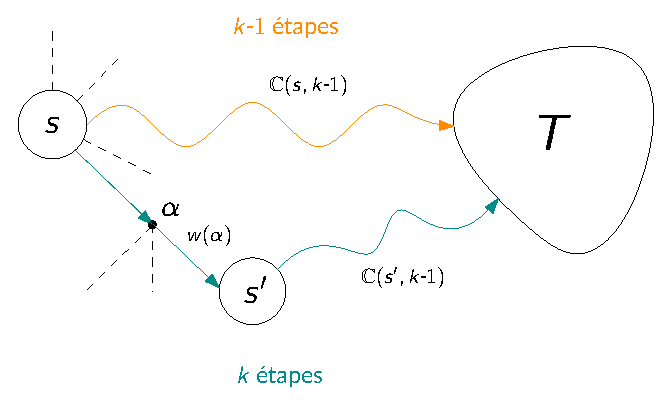
\includegraphics[width=0.6\linewidth]{resources/sp-g}
  \end{center}
\end{frame}

\begin{frame}{SP-G : Programmation dynamique}{Algorithme}
La stratégie $\sigma$ s'il est possible d'atteindre $T$ depuis $s_0$ avec une longueur
de chemin d'au plus $l$ :
\[
  \mathbb{C}(s_0, n) \leq l \iff \exists \sigma, \; \mathbb{P}_{s_0}^\sigma(\Diamond_{\leq l} T) = 1
\]
\begin{center}
  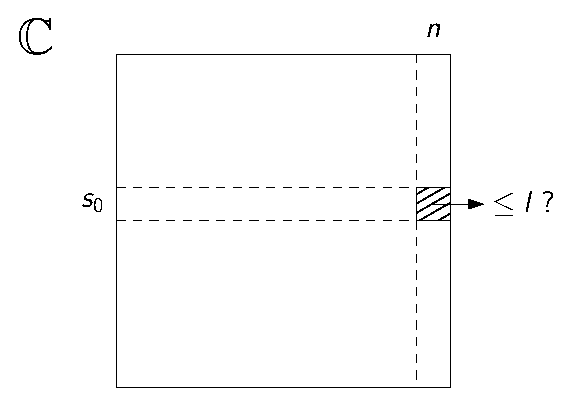
\includegraphics[width=0.4\linewidth]{resources/sp-g2}
\end{center}
\end{frame}

\begin{frame}{SP-G : Programmation dynamique}{Algorithme}
  \textbf{\color{fibeamer@orange}Résumé :}
  \begin{itemize}
    \item $\mathbb{C}(s, k)$ correspond au plus court chemin de $s \in S$ à $T$ après \alert{au plus} $k$ étapes, i.e., après avoir traversé \alert{au plus} $k$ états.
    \item \`A chaque étape, le plus court chemin résulte du choix des actions minimisant, à chaque étape, le coût de la transition menant au \textit{pire} successeur (i.e., celui dont le chemin pour atteindre $T$ est le plus long) est choisit.
    \item Cycle depuis un état $\iff$ on ne peut pas atteindre $T$
    { \color{fibeamer@blue}
    \item $\forall k \in \mathbb{N}, \; \mathbb{C}(s, k-1) \geq \mathbb{C}(s, k)\quad$ pour tout $s \in S$
    %\item Dans le pire cas, le plus court chemin de $s$ à $T$ est celui où tous
    %  les états sont traversés.
    \item $\mathbb{C}(s, n) = \min_k \mathbb{C}(s, k)\quad$ pour tout $s \in S$
    }
  \end{itemize}
\end{frame}

\begin{frame}{SP-G}{Construction de la stratégie}
Soit $s \in S$. Par le fait que
\begin{itemize}
    \item $\forall k \in \mathbb{N}, \; \mathbb{C}(s, k-1) \geq \mathbb{C}(s, k)\quad$ pour tout $s \in S$
    %\item Dans le pire cas, le plus court chemin de $s$ à $T$ est celui où tous
    %  les états sont traversés.
    \item $\mathbb{C}(s, n) = \min_k \mathbb{C}(s, k)\quad$ pour tout $s \in S$
\end{itemize}
On peut construire une stratégie sans mémoire en se basant sur les résultats de $\mathbb{C}(s, n)$ de chaque $s \in S$:
\[
  \sigma : S \rightarrow A, \; s \mapsto arg \min_{\alpha \in A(s)} \max_{s' \in Succ(s, \alpha)} w(\alpha) + \mathbb{C}(s', n)
\]
\end{frame}

\begin{frame}{SP-G}{Construction de la stratégie : intuition}
\small
%\textbf{\color{fibeamer@orange}Idée} : Si $\mathbb{C}(s, n) \neq \infty$, alors
%il existe forcément un état pour lequel passe tel que $\mathbb{C}(s', n) - w(\alpha) = \mathbb{C}(s, n)$

% \begin{itemize}
%     \item $\forall k \in \mathbb{N}, \; \mathbb{C}(s, k-1) \geq \mathbb{C}(s, k)\quad$ pour tout $s \in S$
%     %\item Dans le pire cas, le plus court chemin de $s$ à $T$ est celui où tous
%     %  les états sont traversés.
%     \item $\mathbb{C}(s, n) = \min_k \mathbb{C}(s, k)\quad$ pour tout $s \in S$
% \end{itemize}
Soient $k \in \mathbb{N}, \; s \in S \setminus T$. Supposons que $\mathbb{C}(s, n) \neq \infty$.
\begin{center}
  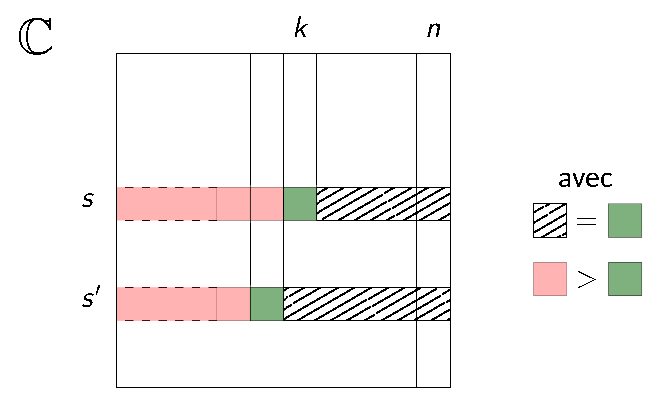
\includegraphics[width=0.5\linewidth]{resources/sp-proof}
\end{center}
\begin{itemize}
  \item $\exists k \leq n$ tel que
$ \mathbb{C}(s, n) = \mathbb{C}(s, k) < \mathbb{C}(s, k-i) \quad \forall i \in \{0, \dots, k\}$ \\
  $\leadsto \; s$ atteint $T$ en $k$ étapes.
  \item $\exists s' \in Succ(s)$ et $\exists \alpha \in A(s)$ tels que $\mathbb{C}(s, k) = \mathbb{C}(s', k-1) + w(\alpha) = \mathbb{C}(s', n) + w(\alpha)$\\
  $\leadsto \; s$ accède à $T$ via $s'$, qui atteint $T$ en $k-1$ étapes.
\end{itemize}

\end{frame}

\begin{frame}{SP-G}{Note}
  \begin{itemize}
    \item poids négatifs : \alert{possible de résoudre en temps pseudo-polynomial}
    \item multi-dimensionnel + poids négatifs : \alert{indécidable}
  \end{itemize}
\end{frame}

\subsection{Exemple}
\begin{frame}{Exemple}{Communication entre noeuds dans un réseau de capteurs}
  \begin{center}
    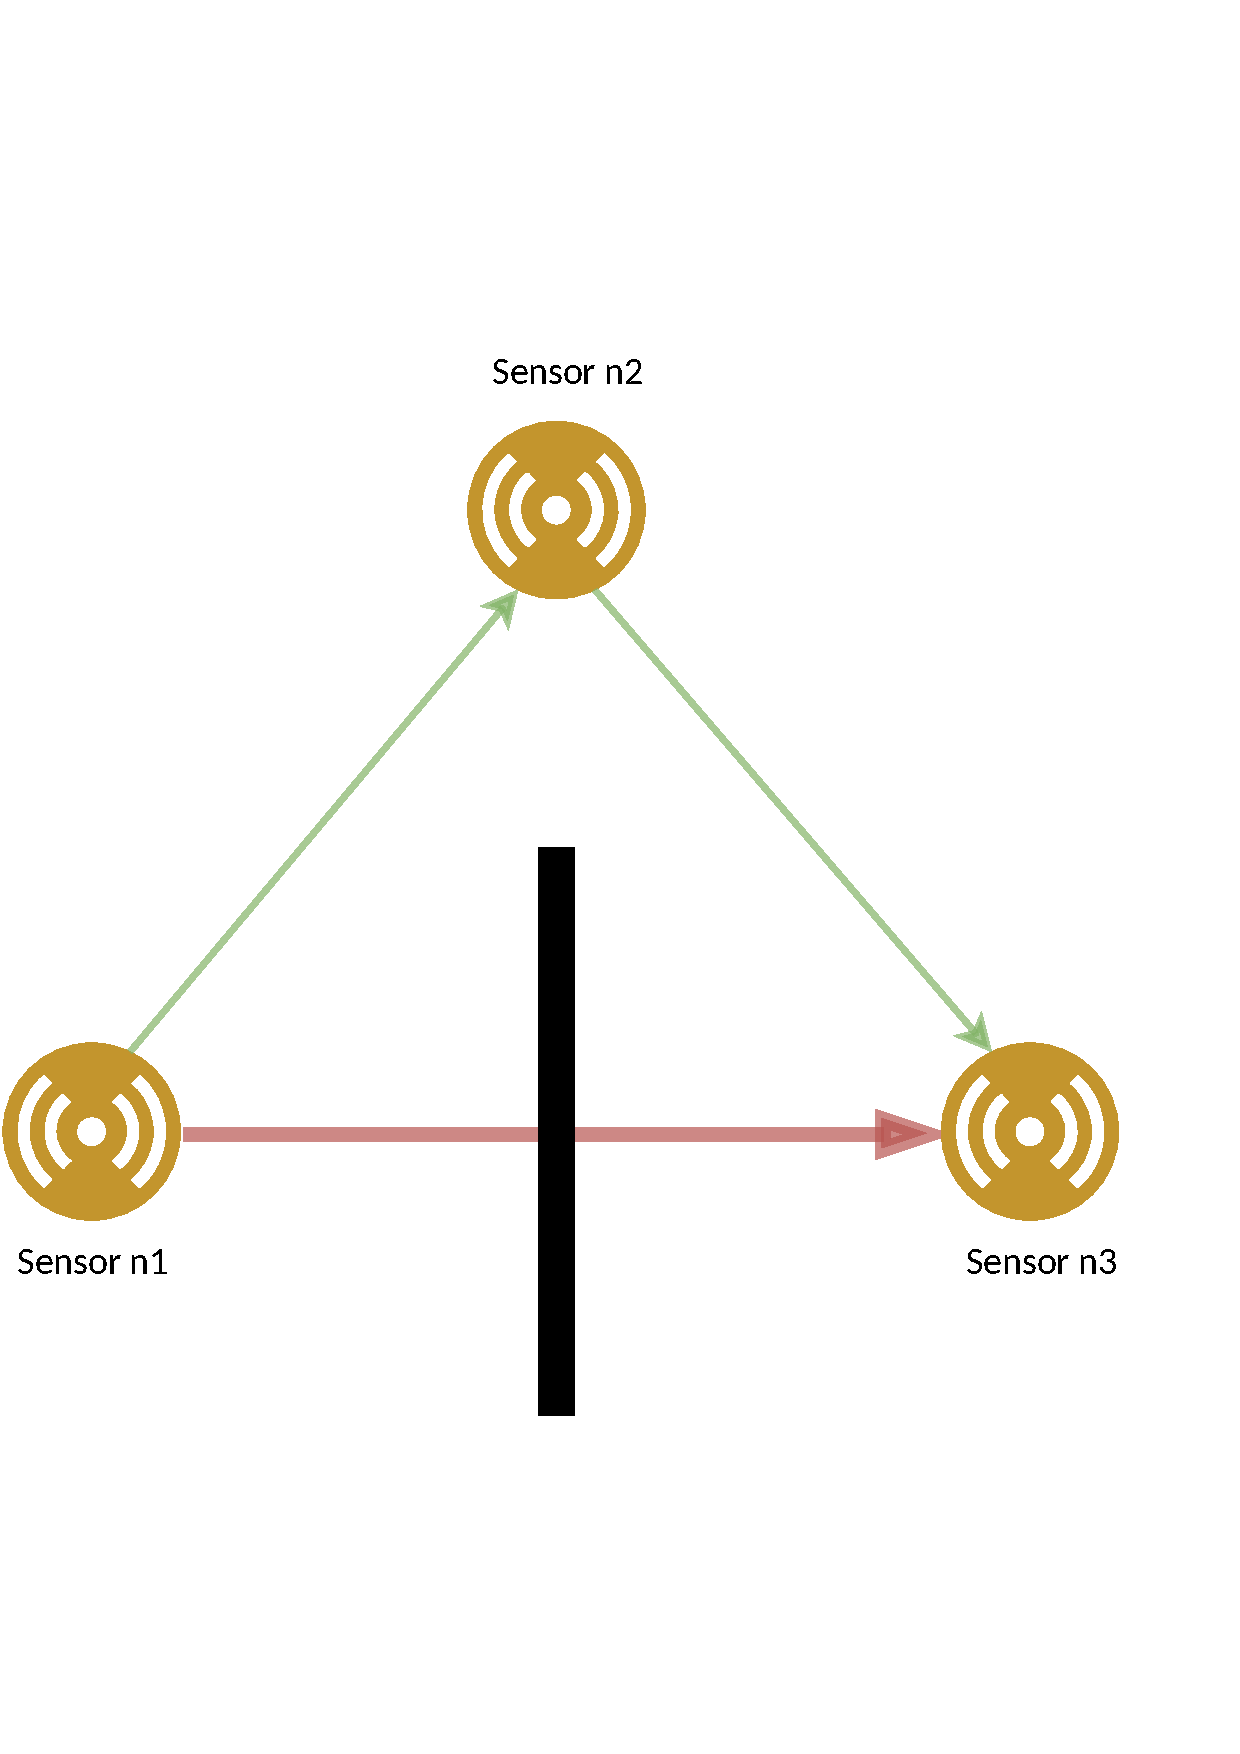
\includegraphics[width=0.65\linewidth]{resources/main-example.pdf}
  \end{center}
\end{frame}

\begin{frame}{Exemple}{Communication entre noeuds dans un réseau de capteurs}
      \begin{itemize}
        \item Un mur sépare $n_0$ et $n_2$
        \item Communication directe $n_0 \rightarrow n_2$
        \begin{itemize}
          \item[$\leadsto$] plus rapide que de passer par un noeud intermédiaire
          \item[$\leadsto$] nécessite plus d'énergie
          \item[$\leadsto$] risque de corruption des paquets envoyés (bruit)
        \end{itemize}
        \item Communication indirecte : $n_0 \rightarrow n_1 \rightarrow n_2$
        \begin{itemize}
          \item[$\leadsto$] plus lent ($n_1$ doit attendre la confirmation de réception du paquet par $n_2$ et $n_0$ doit attendre la confirmation de $n_1$)
          \item[$\leadsto$] consommation d'énergie normale
          \item[$\leadsto$] risque de perte de paquet négligeable
        \end{itemize}
      \end{itemize}
\end{frame}

\begin{frame}{Exemple}{Communication entre noeuds dans un réseau de capteurs}
  \begin{center}
    \only<1>{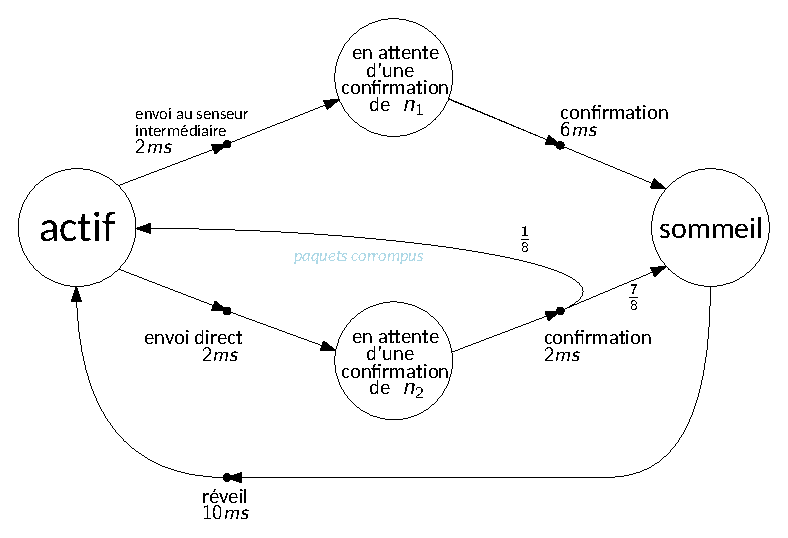
\includegraphics[width=0.7\linewidth]{resources/main-mdp}}
    \only<2>{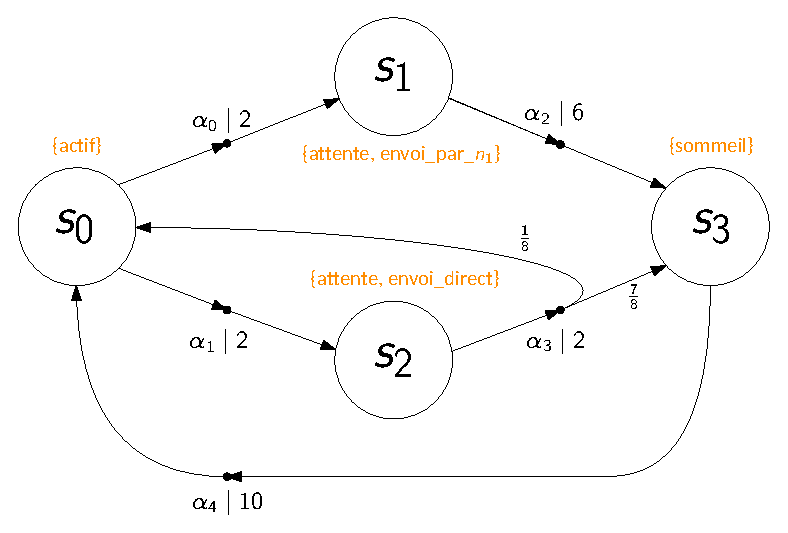
\includegraphics[width=0.7\linewidth]{resources/main-mdp3}}
  \end{center}
\end{frame}

\begin{frame}{Exemple}{Communication entre noeuds dans un réseau de capteurs}
\textbf{Dutty cycle : }$12 ms \; \leadsto \; \exists \sigma, \; \mathbb{P}^\sigma_{s_0}(\Diamond_{\leq 12} \text{ sommeil}) = 1$ ?
\begin{columns}
  \begin{column}{0.5\linewidth}
    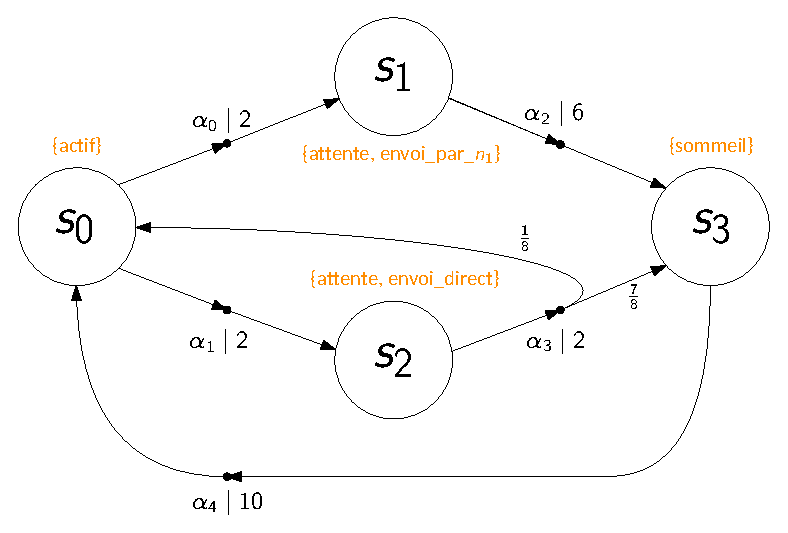
\includegraphics[width=\linewidth]{resources/main-mdp3}
  \end{column}
  \begin{column}{0.5\linewidth}
    \scriptsize
    \begin{itemize}
      \item[$k=0$] \begin{itemize}
        \item $\mathbb{C}(s_0, 0) = \mathbb{C}(s_1, 0) = \mathbb{C}(s_2, 0) = \infty$
        \item $\mathbb{C}(s_3, 0) = 0$
      \end{itemize}
      \item[$k=1$]
        \begin{itemize}
          \item $\mathbb{C}(s_0, 1) = \infty$
          \item $\mathbb{C}(s_1, 1) = 6 + 0 = 6$
          \item $\mathbb{C}(s_2, 1) = 2 + \infty = \infty$
        \end{itemize}
      \item[$k=2$]
        \begin{itemize}
          \item $\mathbb{C}(s_0, 2) = 2 + 6 = 8$
        \end{itemize}
      \item[$k=3$]
        \begin{itemize}
          \item $\mathbb{C}(s_2, 3) = 2 + 8 = 10$
        \end{itemize}
    \end{itemize}
  \end{column}
\end{columns}
\end{frame}

\section{SSP-WE}
\subsection{Motivations}
\begin{frame}{Au delà du pire cas...}
  \begin{itemize}
    \item On souhaite assurer simultanément un {\color{fibeamer@orange}seuil de pire cas} et une {\color{fibeamer@orange}bonne espérance}
  \end{itemize}
  \begin{columns}
    \begin{column}{0.5\linewidth}
      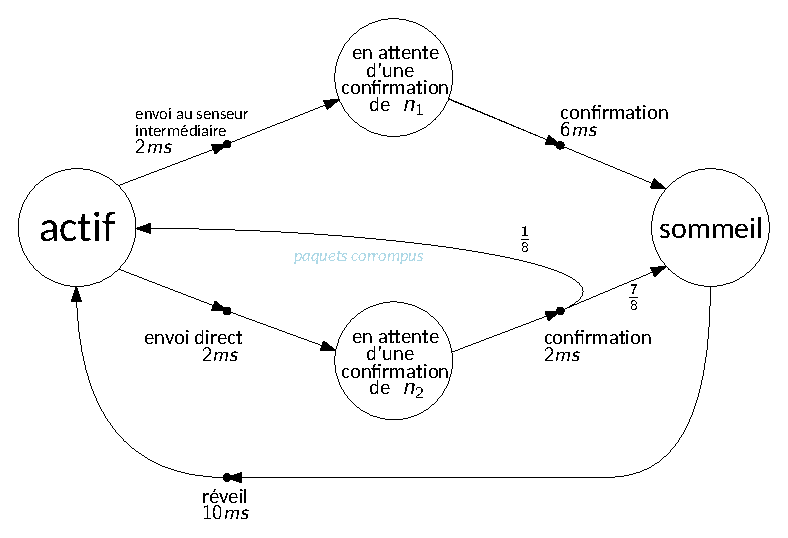
\includegraphics[width=\linewidth]{resources/main-mdp}
    \end{column}
    \begin{column}{0.5\linewidth}
      Quelle est l'espérence optimale du temps d'envoi d'informations au senseur $n_2$ qui assure de respecter le \textit{dutty cycle} du senseur $n_0$ ($12 ms$)  ?
    \end{column}
  \end{columns}
\end{frame}

\subsection{Définition}
\begin{frame}{Espérance sous un pire cas}
  \small
  \begin{definition}[SSP-WE]
    Soient $\mathcal{M}=(S, A, \Delta, w)$, un MDP à une dimension (i.e., tel que $w : A \rightarrow \mathbb{N}_0$), un état initial $s \in S$, un sous-ensemble d'états cibles $T \subseteq S$ et deux seuils $l_1, l_2 \in \mathbb{N}$.
    Le problème consiste à décider s'il existe une stratégie $\sigma$ pour laquelle
    \begin{itemize}
      \item $\forall \pi \in Paths^\sigma(s), \; TS^T(\pi) \leq l_1 \quad
        \equiv \quad \mathbb{P}^\sigma_s(\Diamond_{\leq l_1} T) = 1$
      \item $\mathbb{E}_s^\sigma(\Diamond T) \leq l_2$
    \end{itemize}
  \end{definition}
  \begin{itemize}
    \item décidé en temps {\color{fibeamer@orange}pseudo-polynomial}
    \item NP-hard
    \item mémoire pseudo-polynomiale lors de la construction de la stratégie
  \end{itemize}
\end{frame}

\subsection{Algorithme}
\begin{frame}{SSP-WE}{Algorithme}
  \begin{enumerate}
    \item Construire $\mathcal{M}_{l_1}$, le MDP $\mathcal{M}$ déplié jusque $l_1$
    \item Calculer, $\mathbb{A}$, l'ensemble des actions possibles de l'\textit{\color{fibeamer@orange}attracteur} de $T' = \{ (t, v) \in S_{l_1} \; | \; t \in T \text{ et } v \leq l_1\}$
    \begin{itemize}
      \item[$\leadsto$] pour chaque état $(s, v) \in S_{l_1}$, $\mathbb{A}(s, v)$ est l'ensemble des actions $\alpha \in A(s)$ qui assurent à $(s, v)$ d'atteindre $T'$ dans $\mathcal{M}_{l_1}$, quelle que soit l'issue de l'évolution du système \textit{par l'adversaire} (i.e., l'incertitude lié aux probabilités).
    \end{itemize}
    \item Construire $\mathcal{M}^{\mathbb{A}}_{l_1}$, le MDP déplié limité à l'attracteur de $T'$
    \begin{itemize}
      \item[$\leadsto$] on supprime les états $(s, v)$ de $\mathcal{M}_{l_1}$ tels que $\mathbb{A}(s, v) = \emptyset$
    \end{itemize}
    \item Résoudre le problème SSP-E sur $\mathcal{M}_{l_1}^\mathbb{A}$
  \end{enumerate}
\end{frame}

\begin{frame}{SSP-WE}{Algorithme}
\footnotesize
$\mathbb{A}(s, v)$ peut être calculé récursivement :
\begin{itemize}
  \item \textbf{\color{fibeamer@orange}Idée} : $\mathbb{A}_i(s, v)$ correspond à l'ensemble des actions garantissant au système d'évoluer vers un état sûr (i.e., non-terminal) après $i$ étapes.
  \item $\mathbb{A}_0(s, v) = A(s) \quad $ si $v \leq l$ \\
        $\mathbb{A}_0(s, v) = \emptyset \quad \quad \;$ si $v = \bot$
  \item Soit $i \in \mathbb{N}$. On suppose que $\mathbb{A}_i(s, v)$ a été
    calculé pour tout $(s, v) \in S_{l_1}$. Alors,
\end{itemize}
{
    \[
      \mathbb{A}_{i+1}(s, v) = \{ \alpha \in \mathbb{A}_i(s, v) \; | \;
        \forall (s', v') \in Succ( (s, v), \alpha ), \; \mathbb{A}_i(s', v') \neq \emptyset \}
    \]
}
\begin{center}
  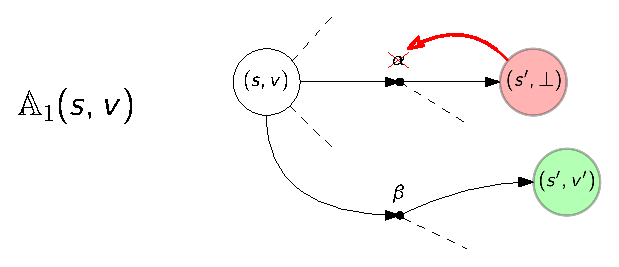
\includegraphics[width=0.5\linewidth]{resources/attractor}
\end{center}
\end{frame}

\begin{frame}{SSP-WE}{Algorithme}
  \begin{itemize}
    \item La taille de l'ensemble $\mathbb{A}_i$ est croissant en $i$, i.e., \\
      $|\mathbb{A}_{i}| \geq |\mathbb{A}_{i+1}| \quad \forall i \in \mathbb{N}$ par définition
    \item Le dépliage du MDP résulte en un DAG
    \begin{itemize}
      \item[$\implies$] pas de cycle !
      \item[$\implies$] le nombre d'itérations $i$ est donc borné par $v$ (= pire cas $\rightarrow$ toutes les actions ont un coût de 1)
      \item[$\implies$] le temps de construction de $\mathbb{A}$ est donc polynomial en la taille du MDP déplié $\mathcal{M}_{l_1} \leadsto \mathcal{O}(v \, \times \, |S_{l_1}|)$
    \end{itemize}
  \end{itemize}
\end{frame}

\begin{frame}{SSP-WE}{Construction de la stratégie}
  $\sigma$ est la stratégie à mémoire finie résultante de la résolution du problème SSP-E sur le MDP $\mathcal{M}_{l_1}^\mathbb{A}$ ($\sigma$ est sans mémoire sur $\mathcal{M}_{l_1}^\mathbb{A}$).
  \begin{itemize}
    \item[$\leadsto$] complexité pseudo-polynomiale
    \item[$\leadsto$] NP-difficile (pas de temps polynomial à moins que P = NP)
  \end{itemize}
\end{frame}

\subsection{Exemple}
\begin{frame}{SSP-WE}{Exemple}
    \[ \overset{?}{\exists} \sigma \; \mathbb{E}^{\sigma}_s(\Diamond \text{ sommeil}) \leq l \wedge \mathbb{P}^\sigma_s(\Diamond_{\leq 12} \text{ sommeil}) = 1 \]
    {\footnotesize Avec $l$, l'espérance minimale pour laquelle le noeud $n_0$ est assuré d'envoyer les données au noeud $n_2$ en moins de $12 ms$ (afin d'assurer un \textit{dutty cycle de $12 ms$}).}
    \begin{center}
      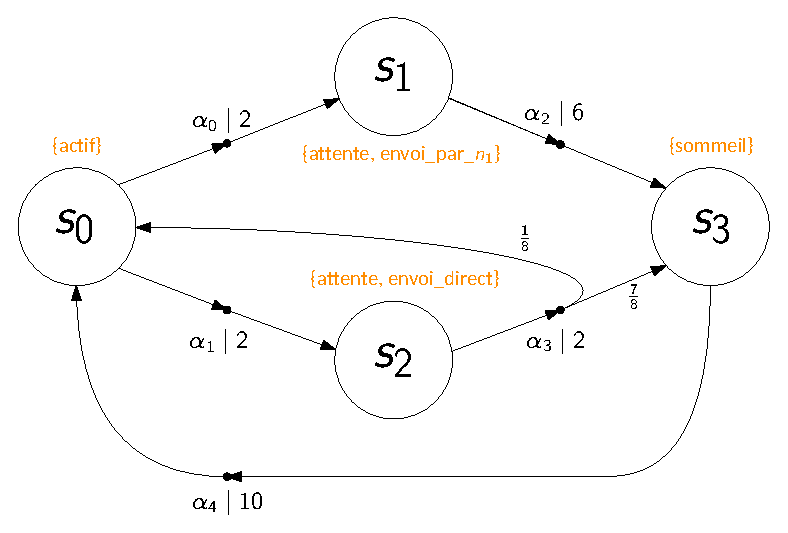
\includegraphics[width=0.6\linewidth]{resources/main-mdp3}
    \end{center}
\end{frame}

\begin{frame}{SSP-WE}{Exemple}
    \[ \overset{?}{\exists} \sigma \; \mathbb{E}^{\sigma}_s(\text{ sommeil}) \leq l \wedge \mathbb{P}^\sigma_s(\Diamond_{\leq 12} \text{ sommeil}) = 1 \]
      \only<1>{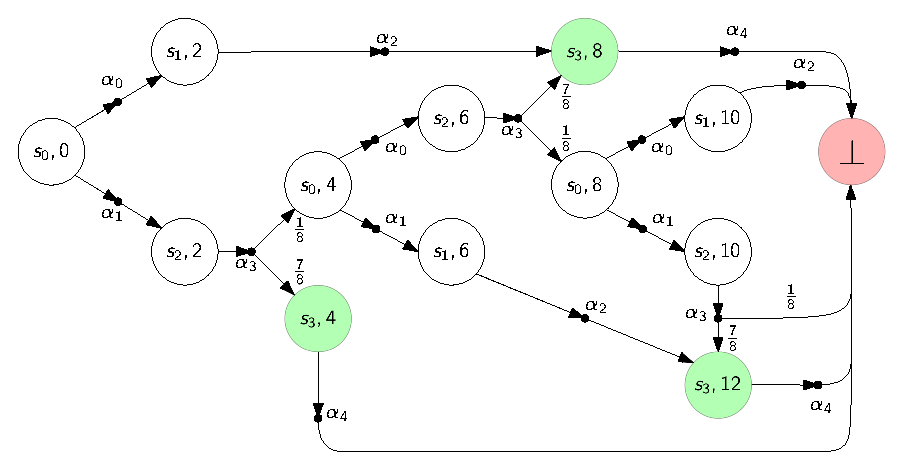
\includegraphics[width=\linewidth]{resources/example-unfolding}}
      \only<2>{
        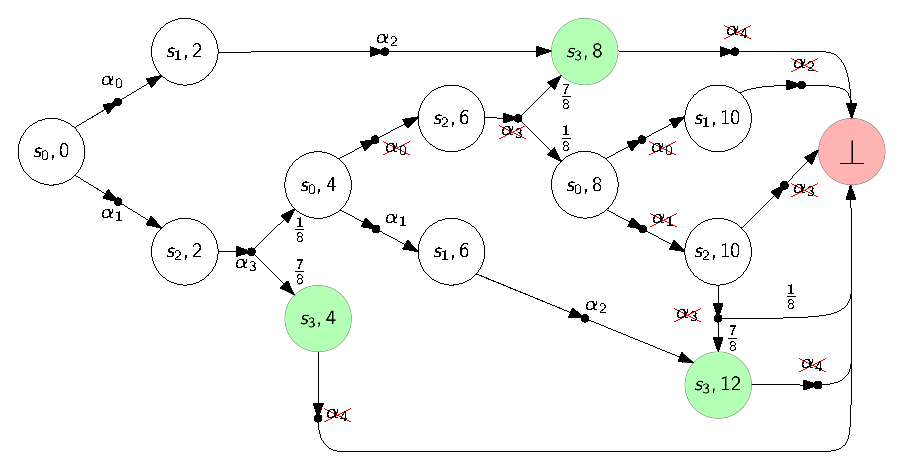
\includegraphics[width=\linewidth]{resources/example-unfoldingA}
      }
\end{frame}

\begin{frame}{SSP-WE}{Exemple}
    \only<1>{\[ \leadsto \mathbb{E}^{\min}_s(\Diamond \{ (s_3, v) \; | \; v \leq 12\}) = ? \]}
    \only<2>{\vspace{-0.02\linewidth}
    \[ \leadsto \mathbb{E}^{\min}_s(\Diamond \{ (s_3, v) \; | \; v \leq 12\}) = \frac{7}{8} \cdot 4 + \frac{1}{8} \cdot 12 = 5 \]}
    \only<1>{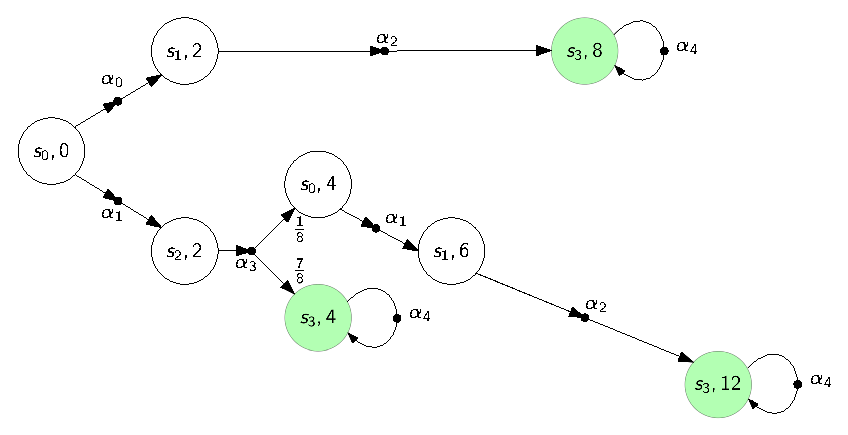
\includegraphics[width=0.96\linewidth]{resources/example-unfoldingA2}}
    \only<2>{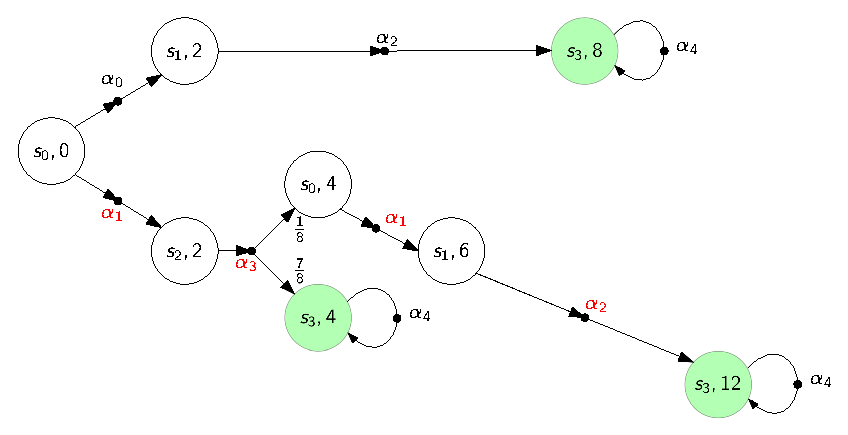
\includegraphics[width=0.96\linewidth]{resources/example-unfoldingA3}}
\end{frame}

\begin{frame}{SSP-WE}{Exemple}
    \vspace{-0.05\linewidth}
    \[ \mathbb{E}^{\sigma}_s(\Diamond \text{ sommeil}) \leq l \wedge \mathbb{P}^\sigma_s(\Diamond_{\leq 12} \text{ sommeil}) = 1 \]
    \begin{center}
      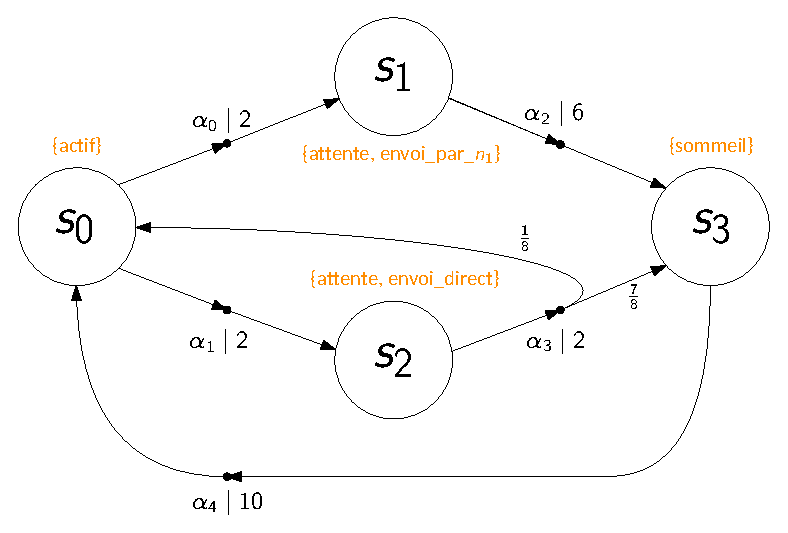
\includegraphics[width=0.6\linewidth]{resources/main-mdp3}
    \end{center}
    \vspace{-0.05\linewidth}
    \begin{itemize}
      \item \textbf{\color{fibeamer@orange}Stratégie optimale $\sigma$} : tester une fois un envoi direct et passer par le noeud $n_1$ si l'envoi direct est un échec.
    \end{itemize}
\end{frame}

\section{SSP-PQ}
\subsection{MDP multidimensionnels}
\begin{frame}{MDP multidimensionnels}
  \begin{definition}[MDP multidimensionnel]
    Un MDP à $d \in \mathbb{N}_0$ dimensions est un tuple $\mathcal{M} = (S, A, \Delta, w)$ tel que
    \begin{itemize}
      \item $S$, $A$, $\Delta$ sont définis de la même façon que pour un MDP classique
      \item $w : A \rightarrow \mathbb{N}_0^d$ est une fonction de coût, associant chaque action à un coût (strictment positif) par dimension du MDP.
    \end{itemize}
  \end{definition}
\end{frame}

\begin{frame}{MDP multidimensionnel}{Exemple}
    On ajoute le coût en énergie de l'envoi d'un message de $n_0$ à $n_2$
  \begin{center}
    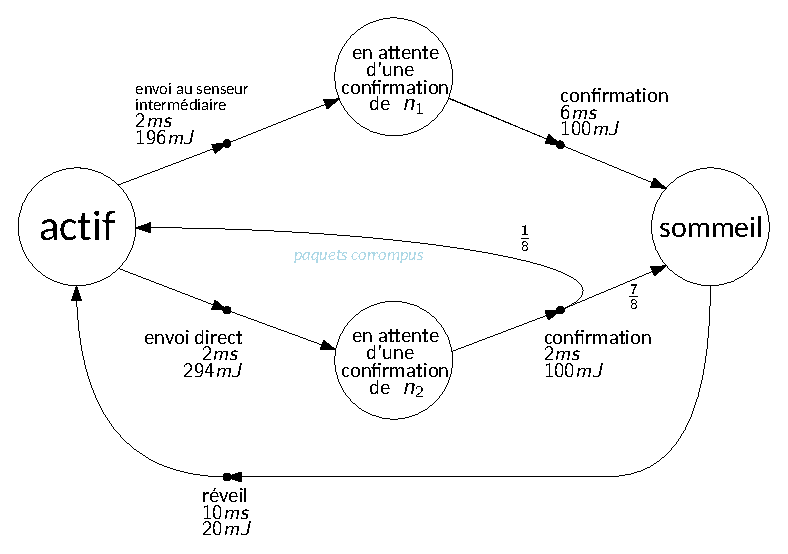
\includegraphics[width=0.7\linewidth]{resources/mdpmdp}
  \end{center}
\end{frame}

\subsection{Motivations}
\begin{frame}{Requêtes percentiles dans les MDP multi-dimensionnels}
  \textbf{\color{fibeamer@orange}Motivation} :
  \begin{itemize}
    \item satisfaire plusieurs requêtes d'accessibilité limité par un coût dans
      un MDP multidimensionnel.
  \end{itemize}
  \begin{center}
    \begin{columns}
      \begin{column}{0.4\linewidth}
        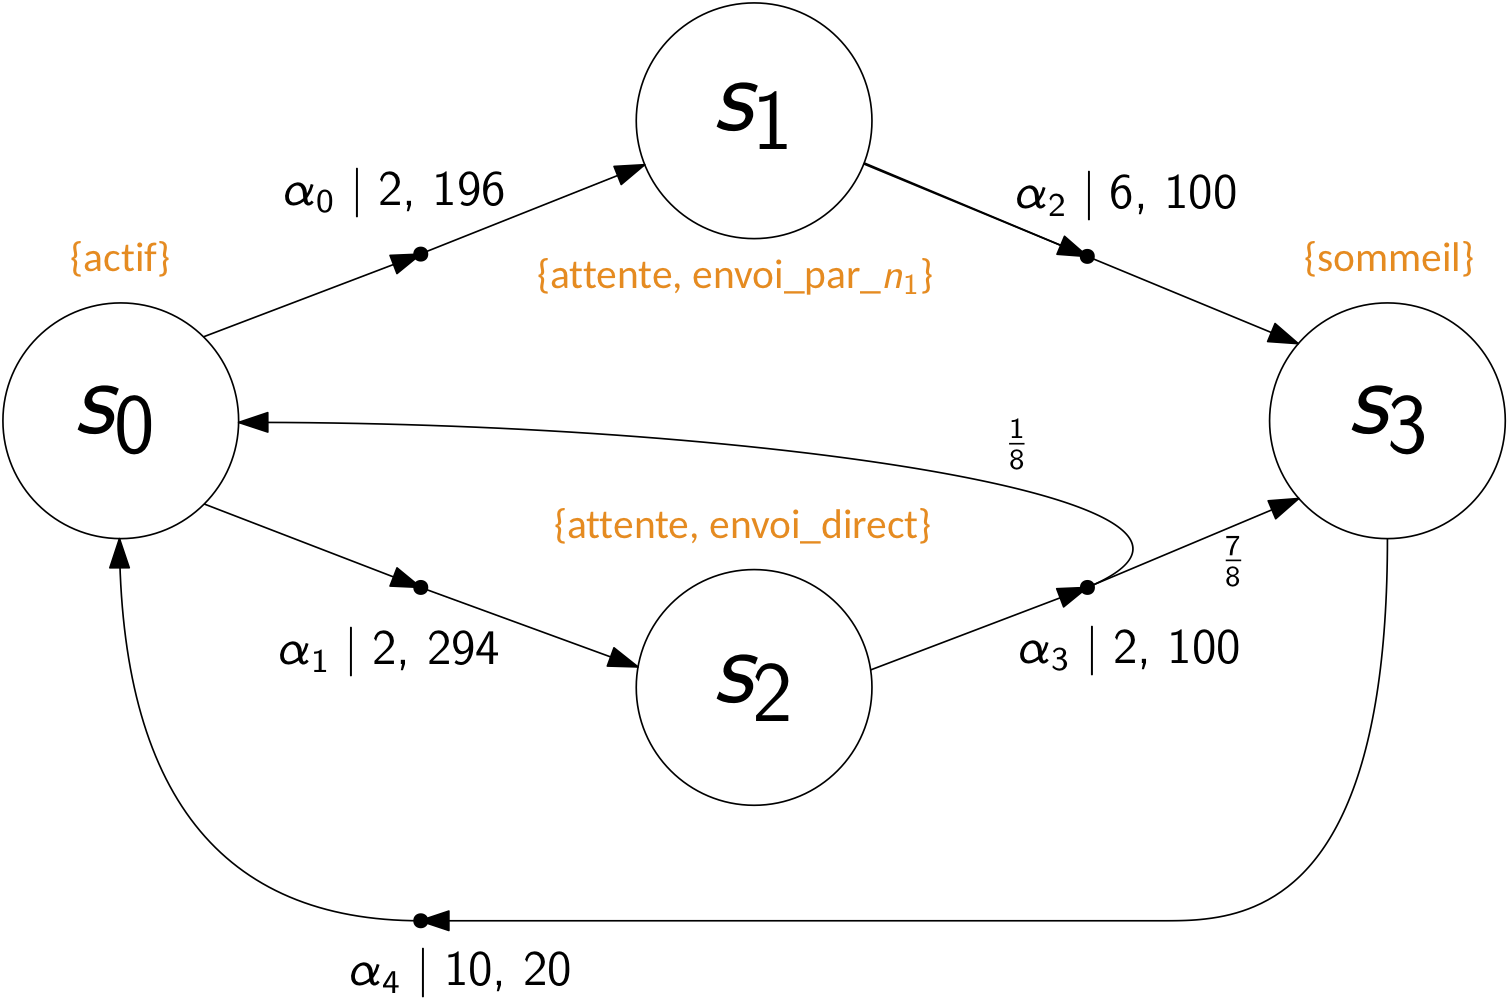
\includegraphics[width=\linewidth]{resources/mdmdp2}
      \end{column}
      \begin{column}{0.6\linewidth}{\small
        \begin{itemize}
          \item $Q_1 := \mathbb{P}^{\sigma_1}_{s_0}(\Diamond_{1\, :\, \leq 4} \text{ sommeil}) \geq 0.8$
          \item $Q_2 := \mathbb{P}^{\sigma_2}_{s_0}(\Diamond_{2\, :\, \leq 700} \text{ sommeil}) \geq 0.9$
            \item[$\leadsto$] $\sigma_1 : $ envoi direct
            \begin{itemize}
              \item[$\implies$] \only<1>{$\mathbb{P}^{\sigma_1}_{s_0}(\Diamond_{1\, :\, \leq 4} \text{ sommeil}) = 0.875$}
              \only<2>{
                ne satisfait pas $Q_2$
              }
            \end{itemize}
            \item[$\leadsto$] $\sigma_2 : $ envoi par un noeud intermédiaire
            \begin{itemize}
              \item[$\implies$] \only<1>{$\mathbb{P}^{\sigma_2}_{s_0}(\Diamond_{2\, :\, \leq 700} \text{ sommeil}) = 1$}
              \only<2>{
                ne satisfait pas $Q_1$
              }
          \end{itemize}
        \end{itemize}
        }
      \end{column}
    \end{columns}
  \end{center}

\end{frame}

\begin{frame}{Requêtes percentiles dans les MDP multi-dimensionnels}
  \textbf{\color{fibeamer@orange}Motivation} :
  \begin{itemize}
    \item satisfaire plusieurs requêtes d'accessibilité limité par un coût dans
      un MDP multidimensionnel.
  \end{itemize}
  \begin{center}
    \begin{columns}
      \begin{column}{0.4\linewidth}
        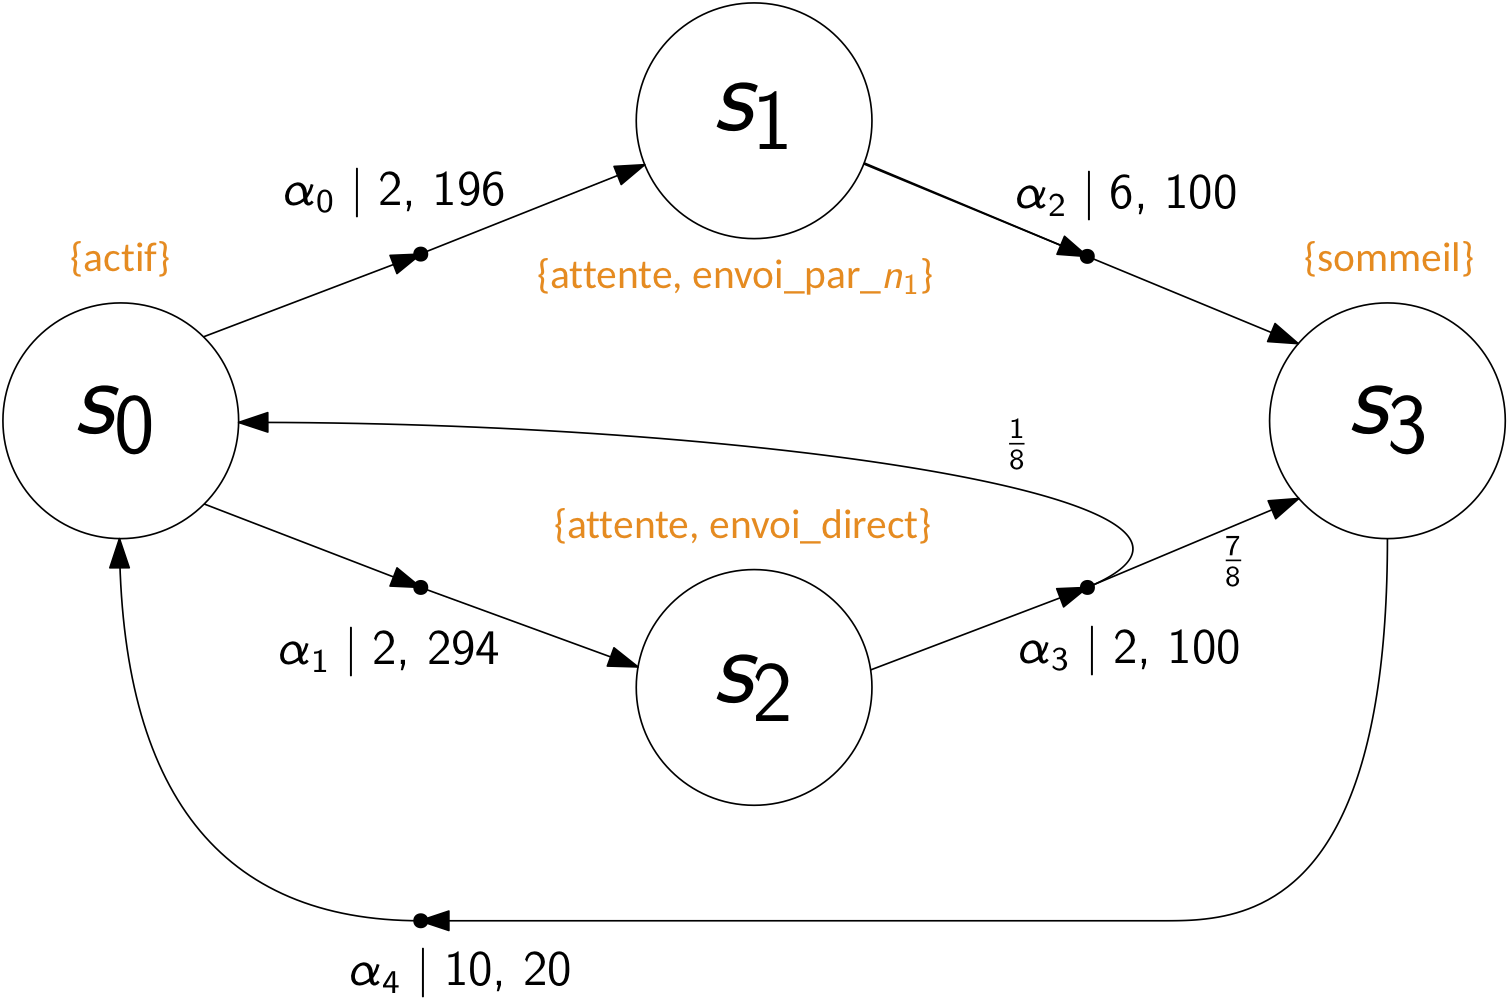
\includegraphics[width=\linewidth]{resources/mdmdp2}
      \end{column}
      \begin{column}{0.6\linewidth}{\small
        \begin{itemize}
          \item $Q_1 := \mathbb{P}^{\sigma_1}_{s_0}(\Diamond_{1\, :\, \leq 4} \text{ sommeil}) \geq 0.8$
          \item $Q_2 := \mathbb{P}^{\sigma_2}_{s_0}(\Diamond_{2\, :\, \leq 700} \text{ sommeil}) \geq 0.9$
        \end{itemize}
        }
      \end{column}
    \end{columns}
  \end{center}
  \begin{itemize}
    \item[$\leadsto$] Résoudre un tel problème requiert une \textit{\color{fibeamer@orange}stratégie à mémoire finie}
  \end{itemize}
\end{frame}

\begin{frame}{Requêtes percentiles dans les MDP multi-dimensionnels}
  \small
      $\sigma_{1 \wedge 2} := $ essayer une fois un envoi direct et passer ensuite par $n_1$ si l'envoi direct a échoué
      \begin{center}
        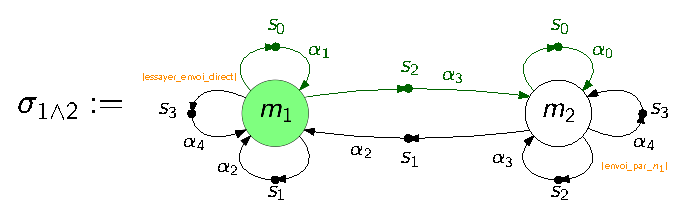
\includegraphics[width=0.7\linewidth]{resources/strategy}
      \end{center}
  \begin{center}
    \begin{columns}
      \begin{column}{0.4\linewidth}
        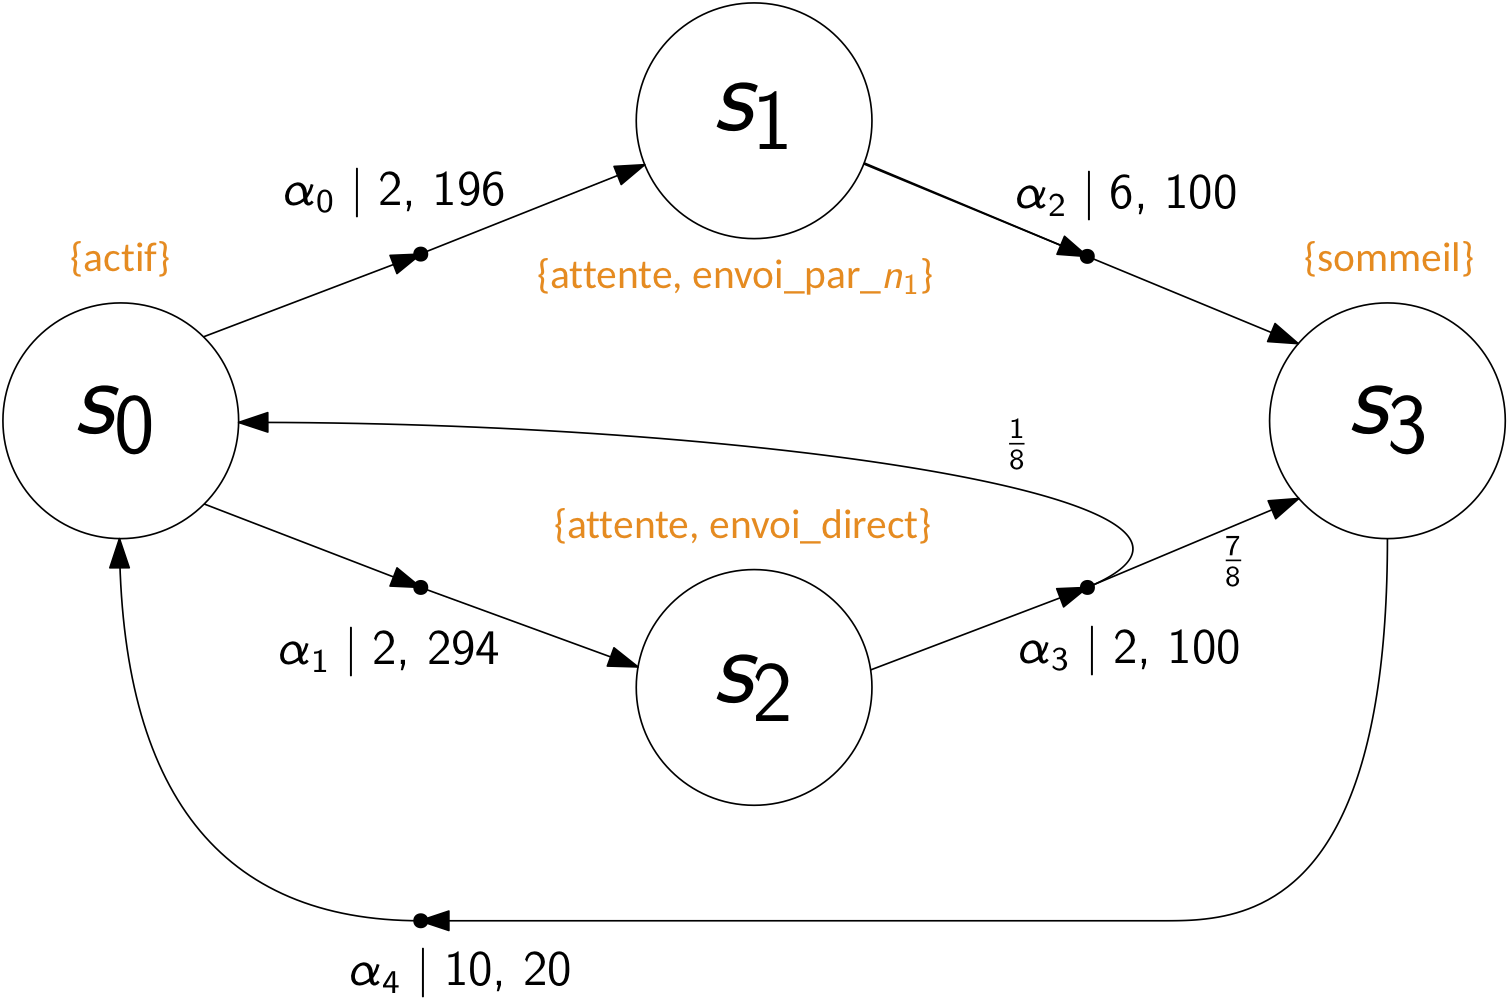
\includegraphics[width=\linewidth]{resources/mdmdp2}
      \end{column}
      \begin{column}{0.6\linewidth}{ \footnotesize
        \begin{itemize}
          \item $Q_1 := \mathbb{P}^{\sigma_{1 \wedge 2}}_{s_0}(\Diamond_{1\, :\, \leq 4} \text{ sommeil}) \geq 0.8$
          \item $Q_2 := \mathbb{P}^{\sigma_{1 \wedge 2}}_{s_0}(\Diamond_{2\, :\, \leq 700} \text{ sommeil}) \geq 0.9$
          \item $\mathbb{P}^{\sigma_{1 \wedge 2}}_{s_0}(\Diamond_{1\, :\, \leq 4} \text{ sommeil}) = 0.875 \models Q_1$
          \item $\mathbb{P}^{\sigma_{1 \wedge 2}}_{s_0}(\Diamond_{2\, :\, \leq 700} \text{ sommeil}) = 1 \models Q_2 $
          \begin{itemize}
            \scriptsize
            \item[$\leadsto$] $394 \leq TS^{\{s_3\}}(\pi) \leq 690$ $\forall \pi \in Paths^{\sigma_{1 \wedge 2}}(s_0)$
          \end{itemize}
        \end{itemize}
        }
      \end{column}
      \end{columns}
      \end{center}
\end{frame}

\begin{frame}{Requêtes percentiles dans les MDP multi-dimensionnels}{Note}
Il est également possible de résoudre ce problème à l'aide d'une stratégie \textit{\color{fibeamer@orange}sans mémoire}, \alert{\textbf{mais}} qui nécessitent de l'\textit{\color{fibeamer@orange}aléatoire} :
\[
  \sigma : A \rightarrow \mathcal{D}(S)
\]
où $\mathcal{D}$ est une distribution de probabilité sur $S$

\end{frame}

\subsection{Définition}
\begin{frame}{SSP-PQ}
  \begin{definition}[SSP-PQ]
    Soient $\mathcal{M} = (S, A, \Delta, w)$, un MDP multidimensionnel tel que
    $w: A \rightarrow \mathbb{N}_0^d$, $s \in S$, un état de $\mathcal{M}$ et $q \in \mathbb{N}$
    contraintes percentiles  par un ensemble d'états cibles
  \end{definition}
\end{frame}

\begin{frame}[allowframebreaks]
        \frametitle{Références}
      \printbibliography
\end{frame}

\end{document}
